\documentclass[12pt]{article}
\usepackage{fullpage}
\usepackage{amsthm}
\usepackage{amsfonts,amsmath, amssymb,latexsym,mathrsfs}
\usepackage[margin=1.15in]{geometry}
\usepackage{enumitem}
\setlength{\parindent}{0pt}
\usepackage{tikz-cd}
\usepackage{fancyhdr}




\theoremstyle{definition}
\newtheorem{thm}{Theorem}[section]

\newtheorem{prop}{Proposition}[section]


\theoremstyle{definition}
\newtheorem{definition}{Definition}[section]

\theoremstyle{remark}
\newtheorem*{remark}{Remark}

\theoremstyle{definition}
\newtheorem{example}{Example}[section]


\theoremstyle{definition}
\newtheorem{lem}{Lemma}[section]


\theoremstyle{definition}
\newtheorem{cor}{Corollary}[section]


\date{}
\title{Exam 2 Summary}


\begin{document}
\maketitle
\section{Work, slicing distances}

Key formula we are using:\\\[
\text{Work done = Force} \cdot \text{Distance}\] or 
\[W=F\cdot s\]

In the setting where we slice the distance, we usually deal with the case of leaking bucket, i.e., mass $m$ is a function of time $t$/a function of distance travelled $h$.
Therefore, we need to slice the distance so we can have $\Delta W=F(h) \cdot \Delta h$.

\section{L'Hopital's rule}

L’Hopital’s rule: If $f$ and $g$ are differentiable and (below $a$ can be $\pm \infty$)\\
i)$f(a) = g(a) = 0$ for finite $a$, \\
Or ii)$\lim_{x\to a} f(x)=\lim_{x\to a} g(x)= \pm \infty$,\\ 
Or iii)$\lim_{x\to \infty} f(x)= \lim_{x\to \infty} g(x) = 0$
then 
\[\lim_{x\to a}\frac{f(x)}{g(x)} = \lim_{x\to a} \frac{f'(x)}{g'(x)} \]

\subsection{Dominance}
We say that $g$ dominates $f$ as $x \to \infty$ if $\lim_{x\to \infty}f(x)/g(x) = 0$. 
\subsection{How to determine some bad limit?}

There are several types of the limits that is ''bad'' which requires L'Hopital's rule to calculate:
$0/0, \infty/\infty, \infty\cdot0$. Although the first two cases we can use L'Hopital's rule to calculate, the others we cannot use it directly.

Read the book, and there are several things that we can consider.
\begin{itemize}
	\item Consider taking log.
	\item Consider $1/f(x)$ so that we can transform $\infty$ to '$1/0$' or $0$ to '$1/\infty$'.
\end{itemize}

\section{Improper integral}
Formal definition of the improper integral I will let you read the book carefully, they are in the box. 
However, informally, there are two types of improper integral which we just interpret them as a limit.

\begin{itemize}
	\item The first case is where we have the limit of the integration goes to infinity, i.e. $\lim_{b \to \infty} \int^b_a f(x) dx$.
	\item The integrand goes to infinity as $x \to a$.
\end{itemize}

\subsection{Converges or diverges?}
The basic question that one want to know about the improper integral is basically is it well defined?

This turns to ask if an improper integral converges or not.

There are four ways people ususally use to check this fact.
\begin{enumerate}
	\item Check by definition, this means check the limit directly.
	\item $p$-test.\\
	\includegraphics*[width=0.9\textwidth]{1.png}
	\item Exponential decay test. 
	\[\int^\infty_0 e^{-ax} dx\] converges for $a>0$.
	\item Comparison test.\\
	If $f(x)\geq g(x) \geq 0$ on the interval $[a,\infty]$ then,\begin{itemize}
	\item If $\int^\infty_a f(x) dx$ converges then so does $\int^\infty_a g(x) dx$.
	\item If $\int^\infty_a g(x) dx$ diverges then so does $\int^\infty_a f(x) dx$.
	\end{itemize}
	\item Limit Comparison theorem.\\
	Limit Comparison Test. If $f(x)$ and $g(x)$ are both positive  on the interval $[a,b)$ where $b$ could be a real number or infinity.
	and
	\[\lim_{x\to b}\frac{f(x)}{g(x)} = C\] such that $0 < C < \infty$
	then the improper integrals $\int^b_a f(x) dx$ and $\int^b_a g(x) dx$ are either both convergent or both divergent.

\end{enumerate}

\section{Probability}
\subsection{PDF and CDF}
\begin{definition}
A function $p(x)$ is a \textbf{probability density function} or PDF if it satisfies the following conditions
\begin{itemize}
\item $p(x) \geq 0$ for all $x$.
\item $\int_{-\infty}^\infty p(x) = 1.$
\end{itemize}
\end{definition}

\begin{definition}
A function $P(t)$ is a \textbf{Cumulative Distribution Function} or cdf, of a density function $p(t)$, is defined by 
\[P(t) =\int_{-\infty}^t p(x) dx \]
Which means that $P(t)$ is the antiderivative of $p(t)$ with the following properties:
\begin{itemize}
\item $P(t)$ is increasing and $0\leq P(t)\leq 1$ for all $t$.
\item $\lim_{t \to \infty}P(t)=1.$
\item $\lim_{t \to -\infty}P(t)=0.$
\end{itemize}
\end{definition}

Moreover, we have $\int_a^b p(x)dx=P(b)-P(a)$.

\subsection{Probability, mean and median}

\subsubsection*{Probability}
Let us denote $X$ to be the quantity of outcome that we care ($X$ is in fact, called the random variable).
\[\mathbb{P}\{a\leq X\leq b\}=\int_a^b p(x)dx=P(b)-P(a)\]
\[\mathbb{P}\{X\leq t\}=\int_{-\infty}^t p(x)dx=P(t)\]
\[\mathbb{P}\{X\geq s\}=\int_{s}^\infty p(x)dx=1-P(s)\]

\subsubsection*{The mean and median}
\begin{definition}
A \textbf{median} of a quantity $X$ is a value $T$ such that the probability of $X\leq T$ is $1/2$. Thus we have  $T$ is defined by the value such that
\[ \int_{-\infty}^T p(x) dx=1/2 \] or \[P(T)=1/2\].
\end{definition}
\begin{definition} A \textbf{mean} of a quantity $X$ is the value given by
	\[ Mean= \frac{\text{Probability of all possible quantity}}{\text{Total probability}}= \frac{\int_{-\infty}^{\infty}xp(x)dx}{\int_{-\infty}^{\infty}p(x)dx}=\frac{\int_{-\infty}^{\infty}xp(x)dx}{1}=\int_{-\infty}^{\infty}xp(x)dx. \]
\end{definition}

\subsubsection*{Normal Distribution}
\begin{definition}
A normal distribution has a density function of the form 
\[p(x)=\frac{1}{\sigma \sqrt{2 \pi}}e^{-\frac{(x-\mu)^2}{2\sigma^2}}\] where $\mu$ is the mean of the distribution and $\sigma$ is the standard deviation, with $\sigma > 0$.
The case $\mu = 0$, $\sigma = 1$ is called the standard normal distribution.

\end{definition}

\section{Sequences and Series}
\subsection{Sequence}
\begin{definition}
	A sequence is an enumerated collection of objects in which repetitions are allowed. We denote the sequence $a_1, a_2, \ldots, a_n \ldots $ as $(a_n)$.

\end{definition}	

Note that for sequence, there are two things that we will usually concern. The first one is the convergence of the sequence itself, which is defined as 

\begin{definition}
The sequence $s_1, s_2, s_3, \ldots , s_n, \ldots$ has a limit $L$, written $\lim_{n \to \infty}s_n = L$, if $s_n$ is as close to
$L$ as we please whenever $n$ is sufficiently large. If a limit, $L$, exists, we say the sequence
converges to its limit $L$. If no limit exists, we say the sequence diverges.
\end{definition}

If we think about the situation more clearly, we will see that, in the definition it actually encodes an information: A convergent sequence is bounded. Is the converse true here? Unfortunately, it is not true that a bounded sequence is convergent. However, by the following theorem, we knows when will the bounded sequence becomes convergent.

\begin{thm}
\textbf{Bounded Monotone sequence converges}: If a sequence $s_n$ is bounded and monotone, it converges.
\end{thm}

\newpage
\subsection{Series}
There is another thing that we will usually concern.

Consider the partial sum of sequence $s_n$, i.e., $S_n=\sum_{i=1}^{n}s_i$, then we will see that the partial sum forms a sequence as well. Therefore there is a natural question to ask here, when will the sequence $S_n$ of partial sums converges?


\begin{definition}
The associated series for a sequence $(a_n)$ is defined as the ordered sum $\sum_{n=1}^{\infty}a_n$.
\end{definition}


\begin{definition}
If the sequence $S_n$ of partial sums converges to $S$, so $\lim_{n \to \infty}S_n = S$, then we say the series
$\sum_{n=1}^{\infty} a_n$ converges and that its sum is $S$. We write
$\sum_{n=1}^{\infty} a_n = S$. If $\lim_{n \to \infty}S_n$ does not exist, we
say that the series diverges.
\end{definition}

There are several properties for convergent series, which is super useful, summarized as below.
\begin{thm}
Convergence Properties of Series
\begin{enumerate}
\item If $\sum_{n=1}^{\infty} a_n$ and $\sum_{n=1}^{\infty} b_n$ converge and if $k$ is a constant, then

$\sum_{n=1}^{\infty} (a_n+b_n)$ converges to$\sum_{n=1}^{\infty} a_n + \sum_{n=1}^{\infty} b_n$.\\
$\sum_{n=1}^{\infty} ka_n$ converges to $k\sum_{n=1}^{\infty} a_n$

\item Changing a finite number of terms in a series does not change whether or not it converges,
\item  If $\lim_{n \to \infty}a_n\neq 0$ or $\lim_{n \to \infty}a_n$ does not exist, then
$\sum_{n=1}^{\infty} a_n$ diverges. (\textbf{Remember this!})
\item If $\sum_{n=1}^{\infty} a_n$ diverges, then $\sum_{n=1}^{\infty} a_n$ diverges if $k\neq 0$.
\end{enumerate}
\end{thm}
\pagebreak
Moreover, there are several test to determine if a series is convergent, detailed discussion about those is in class.
\begin{enumerate}
\item \textbf{The Integral Test}\\
Suppose $a_n = f(n)$, where $f(x)$ is decreasing and positive.
\\a. If $\int_1^\infty f(x) dx$ converges, then $\sum_{n=1}^{\infty} a_n$ an converges.
\\b. If $\int_1^\infty f(x) dx$ diverges, then $\sum_{n=1}^{\infty} a_n$ an diverges.

\item \textbf{p-test}\\
The $p$-series $\sum_{n=1}^{\infty} 1/n^p$ converges if $p > 1$ and diverges if $p \leq 1$.

\item \textbf{Comparison Test}\\
Suppose $0 \leq a_n \leq b_n$ for all $n$ beyond a certain value.
\\ a. If $\sum_{n=1}^{\infty} b_n$ converges, then $\sum_{n=1}^{\infty} a_n$ converges.
\\ b. If $\sum_{n=1}^{\infty} a_n$ diverges, then $\sum_{n=1}^{\infty} b_n$ diverges.

\item \textbf{Limit Comparison Test}\\
Suppose $a_n > 0$ and $b_n > 0$ for all $n$. If
$\lim_{n\to \infty}a_n/b_n= c$ where $c > 0$,
then the two series $\sum_{n=1}^{\infty} a_n$ and $\sum_{n=1}^{\infty} b_n$ either both converge or both diverge.

\item \textbf{Convergence of Absolute Values Implies Convergence}\\
If $\sum_{n=1}^{\infty}|a_n|$ converges, then so does $\sum_{n=1}^{\infty} a_n$.

\item \textbf{The Ratio Test}
For a series $\sum_{n=1}^{\infty} a_n$, suppose the sequence of ratios $|a_{n+1}|/|a_n|$ has a limit:
$\lim_{n\to \infty}|a_{n+1}|/|a_n| = L$, then
\begin{itemize}
\item If $L < 1$, then $\sum_{n=1}^{\infty} a_n$ converges.
\item If $L > 1$, or if $L$ is infinite, then $\sum_{n=1}^{\infty} a_n$ diverges.
\item If $L = 1$, the test does not tell us anything about the convergence of $\sum_{n=1}^{\infty} a_n$ (\textbf{Important!}).
\end{itemize}

\item \textbf{Alternating Series Test}
A series of the form $\sum_{n=1}^{\infty} (-1)^{n-1}a_n = a_1 - a_2 + a_3 - a_4 + \ldots + (-1)^{n-1}a_n + \ldots$
converges if
$0 < a_{n+1} < a_n$ for all $n$ and $lim_{n \to \infty}a_n = 0$.

Error of alternating test: Moreover,  let $S = \lim_{n\to \infty}S_n$, then we will have $|S - S_n| < a_{n+1}$.
\end{enumerate}

Notably, We say that the series $\sum_{n=1}^{\infty} a_n$ is
\begin{itemize}
\item absolutely convergent if $\sum_{n=1}^{\infty} a_n$ and $\sum_{n=1}^{\infty}|a_n|$ both converge.
\item conditionally convergent if $\sum_{n=1}^{\infty} a_n$ converges but $\sum_{n=1}^{\infty}|a_n|$ diverges.
\end{itemize}
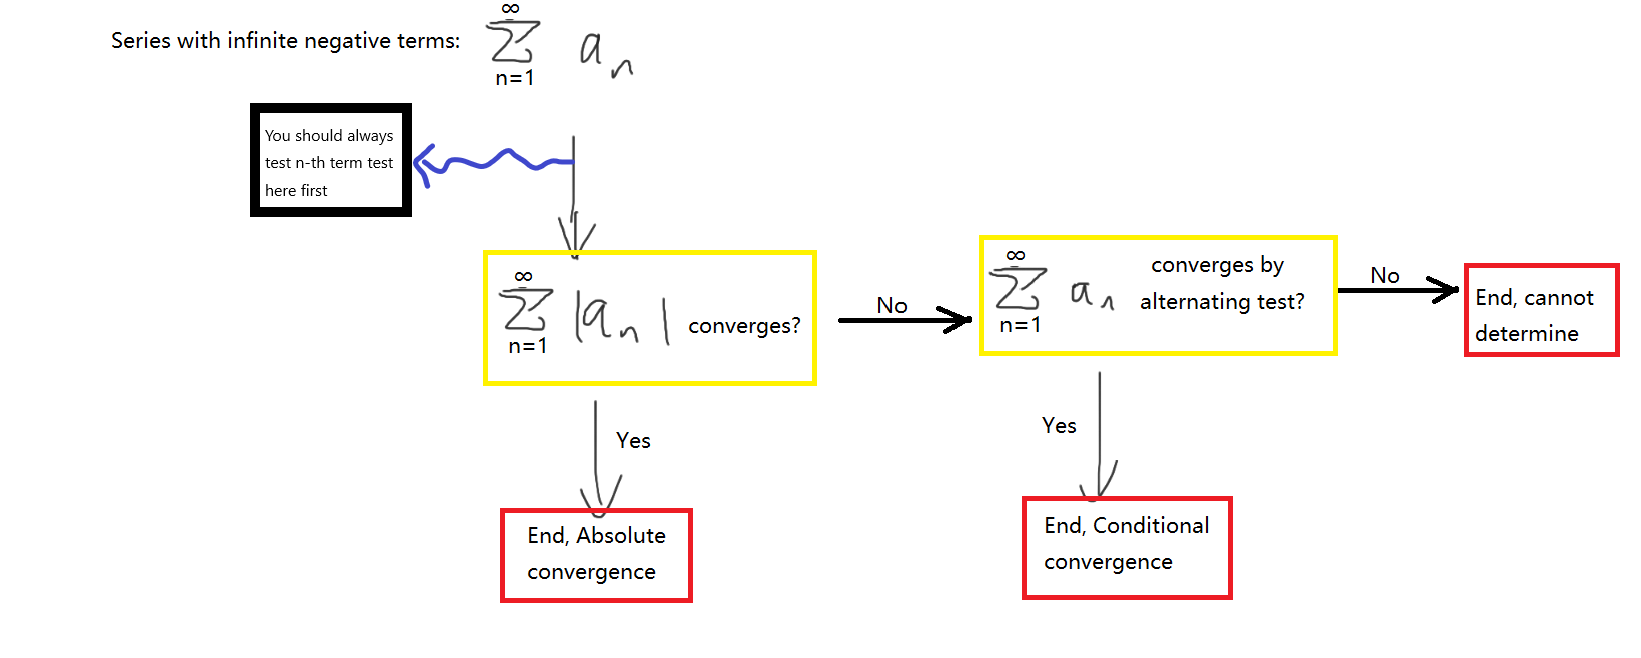
\includegraphics[width=1\textwidth]{program2.png}

Test we consider for proving convergence:
\begin{enumerate}
	\item The integral test
	\item p-test
	\item Comparison test
	\item Limit comparison test
	\item Check the absolute convergence of the series
	\item Ratio Test
	\item Alternating Series Test
\end{enumerate}

Test we consider for proving divergence:
\begin{enumerate}
	\item The integral test
	\item p-test
	\item Comparison test
	\item Limit comparison test
	\item Ratio Test
	\item Check $\lim_{n \to \infty} \neq 0$ or $\lim_{n \to \infty}$ does not exist.
\end{enumerate}

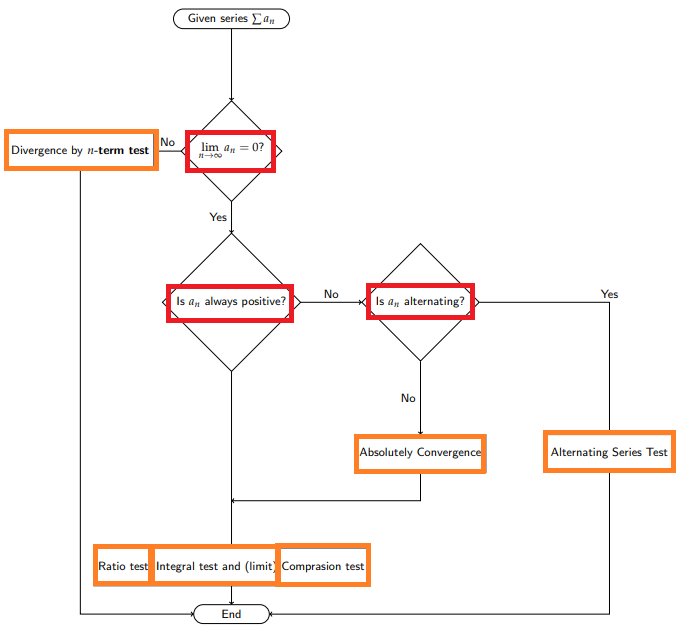
\includegraphics[width=1\textwidth]{program.png}


\subsection{Geometric Series}
There is a special series that we learn about, which is the Geometric Series, notice that the formula on the right hand side is what we called closed form. 
A finite geometric series has the form
\[a + ax + ax^2 + \cdots + ax^{n−2} + ax^{n−1}=\frac{a(1-x^n)}{1-x}\text{ For } x \neq 1\]
An infinite geometric series has the form
\[a + ax + ax^2 + \cdots + ax^{n−2} + ax^{n−1}+ax^n +\cdots=\frac{a}{1-x}\text{ For } |x| < 1\]

\end{document} 